\section{Gestión de la información}

  \paragraph{}Para todas y cada una de las zonas de las que se compone esta
  aplicación (Administrador principal, Administrador de centro, Asesor y
  Alumno), la interfaz compartirá bastantes detalles en común, diferenciándose
  cada una de ellas del resto en el contenido que puede ver y gestionar el
  usuario que está ejecutando la aplicación, teniendo en cuenta el rol con el
  que participa. Por ejemplo, un usuario asesor no podrá ver determinadas zonas
  para la creación de una nueva titulación, ya que es una tarea que no le
  concierne.

  \paragraph{}Teniendo en cuenta lo anterior, a continuación se muestra una
  captura de pantalla para ejemplificar el diseño de la interfaz común a todas
  las zonas de la aplicación. Se ha utilizado la zona del Administrador
  principal por ser la más completa; pero, como se ha comentado antes, el resto
  de zonas comparten los mismos criterios de diseño, por lo cual la
  navegabilidad y usabilidad no varía entre zonas. La figura
  \ref{capturaGestionInformacion} muestra un ejemplo del diseño de la interfaz
  común.

  \begin{figure}[!ht]
    \begin{center}
      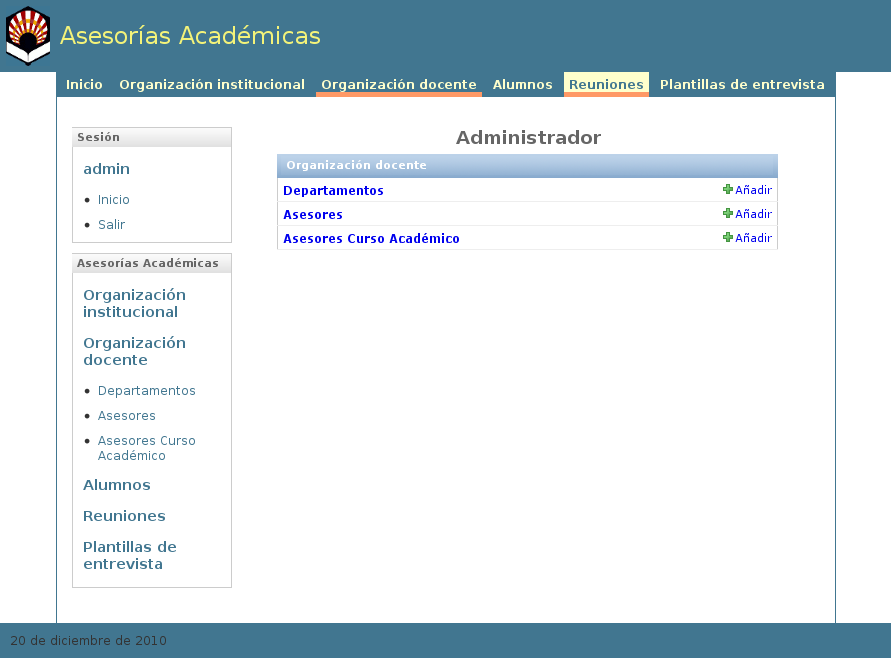
\includegraphics[scale=0.5]{13.Disenyo_Interfaz/13.3.Gestion_Informacion/gestion_informacion.png}
      \caption{Captura de pantalla de la gestión de la información.}
      \label{capturaGestionInformacion}
    \end{center}
  \end{figure}
